\documentclass[aspectratio=169, 10pt]{beamer}

% --- PACKAGES ---
\usepackage[utf8]{inputenc}
\usepackage{tikz}
\usetikzlibrary{shapes.geometric, arrows.meta, positioning, calc}
\usepackage{booktabs}
\usepackage{array}
\usepackage{xcolor}

% --- COLOR PALETTE ---
\definecolor{Ink}{HTML}{1A1D23}
\definecolor{Dim}{HTML}{6B7280}
\definecolor{Accent}{HTML}{2C5F8A}
\definecolor{AccentSoft}{HTML}{EFF3F7}
\definecolor{Line}{HTML}{D8DCE2}
\definecolor{Warn}{HTML}{9A4B3C}
\definecolor{TealAccent}{HTML}{2C5F8A}
\definecolor{AmberAccent}{HTML}{D97706}
\definecolor{CardBg}{HTML}{F8FAFC}
\definecolor{TextDim}{HTML}{6B7280}

% --- BEAMER THEME CUSTOMIZATION ---
\setbeamercolor{background canvas}{bg=white}
\setbeamercolor{normal text}{fg=Ink}
\setbeamercolor{title}{fg=Ink}
\setbeamercolor{subtitle}{fg=Dim}
\setbeamercolor{author}{fg=Dim}
\setbeamercolor{date}{fg=Dim}
\setbeamercolor{item}{fg=Accent}
\setbeamercolor{subitem}{fg=Dim}
\setbeamercolor{block title}{bg=AccentSoft, fg=Accent}
\setbeamercolor{block body}{bg=white, fg=Ink}
\setbeamertemplate{itemize items}[circle]
\setbeamertemplate{navigation symbols}{}
\setbeamertemplate{blocks}[rounded][shadow=false]
\setlength{\parskip}{0pt}

% Frametitle template with subtitle support
\setbeamertemplate{frametitle}{
  \vspace{0.25cm}
  {\large\bfseries\color{Ink}\insertframetitle\par}
  \ifx\insertframesubtitle\empty
  \else
    \vspace{1pt}
    {\footnotesize\color{Dim}\insertframesubtitle\par}
  \fi
  \vspace{3pt}
  {\color{Line}\rule{\linewidth}{0.6pt}\par}
  \vspace{4pt}
}

\setbeamertemplate{footline}{
  \hfill\raisebox{6pt}{\color{Dim}\scriptsize\insertframenumber\,/\,\inserttotalframenumber}\hspace*{24pt}\vspace{4pt}
}

\setbeamertemplate{title page}{
  \vspace{2.2cm}
  {\color{Line}\rule{\linewidth}{0.6pt}}\\[0.5cm]
  {\centering\Huge\bfseries\color{Ink}\inserttitle\par}
  \vspace{0.25cm}
  {\centering\large\color{Accent}\insertsubtitle\par}
  \vspace{0.6cm}
  {\centering\normalsize\color{Dim}\insertauthor\par}
  \vspace{0.15cm}
  {\centering\normalsize\color{Dim}\insertdate\par}
  \vspace{0.4cm}
  {\color{Line}\rule{\linewidth}{0.6pt}}
}

% --- METADATA ---
\title{ROTATING LED DISPLAY}
\subtitle{Wireless Control \& Persistence of Vision (POV) Platform}
\author{ATmega32-Based Embedded Systems Design \\ Student IDs: 2205139, 2205143, 2205147}
\date{Project Proposal \& Technical Architecture}

\begin{document}

% --- SLIDE 1: TITLE ---
\begin{frame}
    \titlepage
\end{frame}

% --- SLIDE 2: MOTIVATION - PROBLEM DESCRIPTION & IMPORTANCE ---
\begin{frame}{1. Motivation}{Problem Description \& Importance}
    \begin{columns}[T]
        \begin{column}{0.48\textwidth}
            \begin{block}{Problem Description}
                \small
                \begin{itemize}
                    \item Traditional flat electronic displays (LCD/OLED/LED matrices) require large physical footprints, heavy mounting frames, and high component counts.
                    \item Viewing angle limitations restrict visibility in 360$^\circ$ public environments or cylindrical installations.
                    \item Displaying dynamic text and real-time graphics on a rotating body creates complex synchronization challenges due to mechanical jitter and phase drift.
                \end{itemize}
            \end{block}
        \end{column}
        \begin{column}{0.48\textwidth}
            \begin{block}{Why It Matters}
                \small
                \begin{itemize}
                    \item Persistence of Vision (POV) technology exploits human visual latency ($\approx$100 ms retention) to render high-resolution 360$^\circ$ displays using only a single spinning array of LEDs.
                    \item Drastically reduces cost, weight, power, and component count compared to multi-panel display grids.
                    \item Demonstrates real-time microsecond-level embedded timing, precise external interrupt synchronization, and multi-protocol wireless integration.
                \end{itemize}
            \end{block}
        \end{column}
    \end{columns}
\end{frame}

% --- SLIDE 3: MOTIVATION - WHY THIS PROJECT & OBJECTIVES ---
\begin{frame}{1. Motivation}{Why This Project \& Main Objectives}
    \footnotesize The project combines high-speed motor rotation, microsecond-accurate LED blinking, real-time wireless Bluetooth communication, RTC timekeeping, and interrupt-driven phase locking on the ATmega32 microcontroller to build a floating cylindrical POV display.
    \vspace{0.05cm}
    \begin{enumerate}
        \footnotesize
        \item \textbf{High-Resolution POV Rendering:} Blink a 24-LED array with microsecond precision during rotation to generate crisp alphanumeric characters, digital clocks, and analog clock hands without visual flicker.
        \item \textbf{Interrupt-Based Phase Synchronization:} Interface an IR obstacle sensor with external interrupt hardware (INT0) to detect rotation cycle completion and eliminate display drift/rotation.
        \item \textbf{Real-Time Clock Synthesis:} Integrate a DS3231 RTC module over I$^2$C (TWI) to display continuous analog (hour/minute/second hands across 60 angular ticks) and digital clocks.
        \item \textbf{Wireless Dynamic Telemetry:} Receive custom text strings over Bluetooth (HC-05 hardware USART) and render them on-the-fly without interrupting rotation phase locking.
        \item \textbf{Onboard Power Autonomy:} Implement a 3.7 V Li-Ion battery power circuit with onboard charging to eliminate trailing wires on the spinning arm.
    \end{enumerate}
\end{frame}

% --- SLIDE 4: MOTIVATION - REAL-WORLD APPLICATION SCENARIOS ---
\begin{frame}{1. Motivation}{Real-World Deployment Scenarios}
    \tiny
    \begin{table}
        \centering
        \begin{tabular}{p{2.7cm} p{3.0cm} p{5.3cm}}
            \toprule
            \textbf{\color{Accent} Operational Sector} & \textbf{\color{Accent} Technical Challenge} & \textbf{\color{Accent} POV Platform Solution} \\
            \midrule
            360$^\circ$ Cylindrical Public Advertising & Multi-panel displays have dead spots and high power draw & Single spinning LED arm renders seamless 360$^\circ$ cylindrical text/logos with 90\% power savings. \\
            Compact Public Information Kiosks & Limited enclosure space for bulky multi-digit LED displays & High-speed rotating PCB projects floating digital/analog clocks and live notifications in a compact footprint. \\
            Industrial Event Telemetry & Cable entanglement on rotating machinery & Onboard Li-Ion battery power + wireless HC-05 Bluetooth serial link streams real-time messages cable-free. \\
            \bottomrule
        \end{tabular}
    \end{table}
    \vspace{0.1cm}
    {\tiny\color{TextDim} All scenarios run on the same core interrupt-driven FSM -- only incoming Bluetooth commands and display modes differ.}
    \vspace{0.1cm}
    \footnotesize
    \begin{itemize}
        \item \textbf{Visual Efficiency:} Uses visual memory to transform a 1D line of 24 LEDs into a 2D cylindrical surface display.
        \item \textbf{Dynamic Remote Reconfiguration:} Bluetooth wireless interface allows operators to update displayed text instantly from any mobile terminal.
        \item \textbf{Hardware Integrity:} Self-contained battery power supply avoids slip-ring noise and mechanical brush wear.
    \end{itemize}
\end{frame}

% --- SLIDE 5: EQUIPMENT - COMPONENT TABLE ---
\begin{frame}{2. Equipment}{Hardware Components \& Justification}
    \tiny
    \renewcommand{\arraystretch}{0.93}
    \begin{table}
        \centering
        \begin{tabular}{p{2.15cm} p{2.85cm} p{5.6cm}}
            \toprule
            \textbf{\color{Accent} Component} & \textbf{\color{Accent} Specification / Count} & \textbf{\color{Accent} Purpose \& Justification} \\
            \midrule
            Microcontroller & ATmega32-16PU (DIP-40) $\times$1 & Core system controller. Provides 32 GPIO lines for 24-LED direct port control, hardware INT0 for IR phase anchor, USART for HC-05, and TWI for DS3231 RTC. \\
            LED Array & High-Brightness 5mm LEDs $\times$24 & Primary visual display element mounted on the spinning panel; lit in bit-pattern columns to form text and clock hands. \\
            Phase Anchor Sensor & IR Obstacle Sensor Module $\times$1 & Positioned at fixed frame anchor; triggers external interrupt (INT0) once per rotation to reset phase counter and eliminate image drift. \\
            Wireless Module & HC-05 Bluetooth Module $\times$1 & Interfaces with hardware USART (PD0/PD1) to receive custom text strings wirelessly from smartphones or PCs. \\
            Real-Time Clock & DS3231 RTC Module $\times$1 & High-precision I$^2$C RTC module; provides real-time timekeeping for analog clock (60 angular slots) and digital clock display. \\
            Drive Motor & High-RPM DC Motor $\times$1 & Rotates the LED panel at stable RPM ($\ge 1000$ RPM) to achieve visual persistence above 15--20 Hz frame rate. \\
            Power Circuit & 3.7V Li-Ion + Charging Module $\times$1 & Onboard battery mounted directly on spinning PCB, providing wireless power to LEDs and MCU without heavy slip rings. \\
            Stationary Power & 5V Wall Charger $\times$1 & Bench power supply for motor drive unit and stationary battery charger circuit. \\
            \bottomrule
        \end{tabular}
    \end{table}
\end{frame}

% --- SLIDE 6: EQUIPMENT - CONTROLLER EVALUATION: NANO VS ATMEGA32 ---
\begin{frame}{2. Equipment}{Microcontroller Evaluation: Arduino Nano vs. ATmega32}
    \tiny
    \begin{table}
        \centering
        \begin{tabular}{p{2.2cm} p{2.3cm} p{2.5cm} p{3.9cm}}
            \toprule
            \textbf{\color{Accent} Metric / Feature} & \textbf{\color{Accent} Arduino Nano (ATmega328P)} & \textbf{\color{Accent} ATmega32-16PU (Selected)} & \textbf{\color{Accent} Justification \& Feature Preserving Verdict} \\
            \midrule
            GPIO Count & 22 Digital/Analog Pins & \textbf{32 Dedicated I/O Lines} & ATmega32 provides 4 full 8-bit ports (PA, PB, PC, PD). Direct 24-LED driving without external multiplexer shift registers. \\
            Port Writing Speed & Multi-pin bit shifting required & \textbf{Single-cycle 8-bit PORT write} & Writing \texttt{PORTA}, \texttt{PORTB}, \texttt{PORTC} in 1 clock cycle gives ultra-sharp LED column switching for high-RPM spinning. \\
            UART Baud Precision & Subject to clone bootloader baud bug (38400 $\rightarrow$ 9600 mismatch) & \textbf{0.0\% Baud Error with 11.0592 MHz crystal} & Eliminates the market-clone Arduino Nano hardware baud error reported in early testing; ensures reliable 115200/38400 Bluetooth transfers. \\
            Hardware Interfaces & 1$\times$ SPI, 1$\times$ I$^2$C, 1$\times$ USART, 2$\times$ Ext Int & \textbf{1$\times$ SPI, 1$\times$ TWI, 1$\times$ USART, 3$\times$ Ext Int} & Retains 100\% functionality (USART for HC-05, TWI for DS3231, INT0 for IR sensor) while offering 10 extra GPIO pins and native 40-pin socketing. \\
            Is Nano Mandatory? & Convenience dev-board & \textbf{NOT strictly mandatory} & Moving to ATmega32 retains 100\% features, improves execution timing, and satisfies academic embedded system criteria. \\
            \bottomrule
        \end{tabular}
    \end{table}
    \vspace{0.1cm}
    \footnotesize\color{Dim} \textbf{Conclusion:} Arduino Nano is NOT strictly mandatory. Moving to ATmega32 preserves all capabilities, fixes serial baud mismatches, and simplifies 24-LED driving via full 8-bit port registers.
\end{frame}

% --- SLIDE 7: EQUIPMENT - SOFTWARE ---
\begin{frame}{2. Equipment}{Software \& Development Tools}
    \begin{columns}[T]
        \begin{column}{0.5\textwidth}
            \begin{block}{Toolchain \& Compilers}
                \small
                \begin{itemize}
                    \item \textbf{Microchip Studio / AVR-GCC} -- Bare-metal C development, register-level drivers, and hex generation.
                    \item \textbf{USBasp Programmer \& eXtreme Burner} -- Direct ISP flashing into ATmega32 Flash memory.
                    \item \textbf{Proteus VSM} -- Full circuit schematic design and timing simulation before PCB fabrication.
                \end{itemize}
            \end{block}
        \end{column}
        \begin{column}{0.5\textwidth}
            \begin{block}{Host \& Testing Software}
                \small
                \begin{itemize}
                    \item \textbf{Serial Bluetooth Terminal (Android / PC)} -- Wireless transmission of custom ASCII strings to HC-05.
                    \item \textbf{Custom Bit-Matrix Generator} -- Python/C utility to map ASCII characters into 8$\times$5 and 24$\times$5 LED column matrices.
                \end{itemize}
            \end{block}
        \end{column}
    \end{columns}
    \vspace{0.2cm}
    \footnotesize\color{Dim} The ATmega32 handles phase detection, timing delays, bit pattern output, and RTC reads autonomously. The Bluetooth terminal is strictly an input medium.
\end{frame}

% --- SLIDE 8: SYSTEM DESIGN - BLOCK DIAGRAM ---
\begin{frame}{3. System Design}{System Hardware Block Diagram}
    \centering
    \resizebox{0.98\textwidth}{!}{
        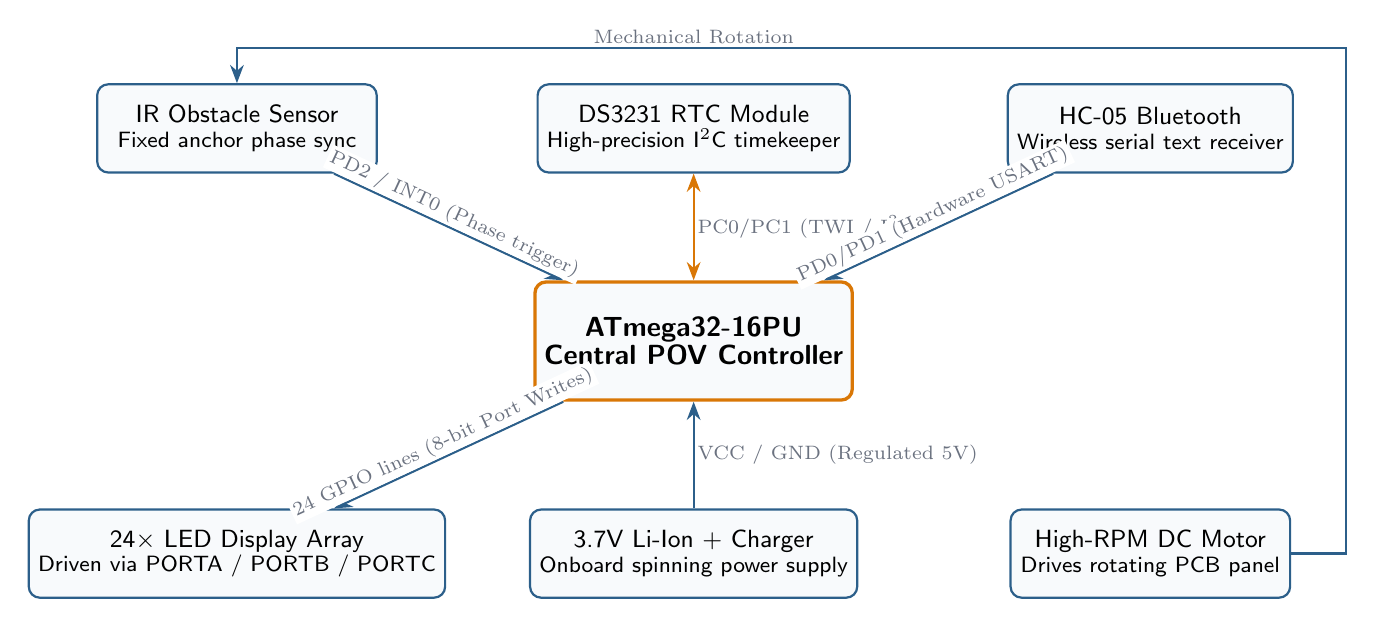
\begin{tikzpicture}[
            mcu/.style={rectangle, draw=AmberAccent, very thick, fill=CardBg, rounded corners, minimum height=1.5cm, minimum width=3.8cm, align=center, font=\sffamily\bfseries\normalsize},
            block/.style={rectangle, draw=TealAccent, thick, fill=CardBg, rounded corners, minimum height=1.12cm, minimum width=3.55cm, align=center, font=\sffamily\small},
            smallblock/.style={rectangle, draw=Line, thick, fill=white, rounded corners, minimum height=0.95cm, minimum width=3.3cm, align=center, font=\sffamily\scriptsize},
            arrow/.style={-Stealth, thick, color=TealAccent},
            biarrow/.style={Stealth-Stealth, thick, color=AmberAccent},
            lbl/.style={font=\scriptsize, color=TextDim, fill=white, inner sep=1pt}
        ]
            % Input / Sensor Layer
            \node[block] (ir) at (-5.8,2.7) {IR Obstacle Sensor\\[-2pt]\footnotesize Fixed anchor phase sync};
            \node[block] (rtc) at (0,2.7) {DS3231 RTC Module\\[-2pt]\footnotesize High-precision I$^2$C timekeeper};
            \node[block] (bt) at (5.8,2.7) {HC-05 Bluetooth\\[-2pt]\footnotesize Wireless serial text receiver};

            % Central controller
            \node[mcu] (mcu) at (0,0) {ATmega32-16PU\\[-2pt]\normalsize Central POV Controller};

            % Output / Power Layer
            \node[block] (leds) at (-5.8,-2.7) {24$\times$ LED Display Array\\[-2pt]\footnotesize Driven via PORTA / PORTB / PORTC};
            \node[block] (power) at (0,-2.7) {3.7V Li-Ion + Charger\\[-2pt]\footnotesize Onboard spinning power supply};
            \node[block] (motor) at (5.8,-2.7) {High-RPM DC Motor\\[-2pt]\footnotesize Drives rotating PCB panel};

            % Connections
            \draw[arrow] (ir) -- node[lbl, above, sloped]{PD2 / INT0 (Phase trigger)} (mcu);
            \draw[biarrow] (rtc) -- node[lbl, right]{PC0/PC1 (TWI / I$^2$C)} (mcu);
            \draw[arrow] (bt) -- node[lbl, above, sloped]{PD0/PD1 (Hardware USART)} (mcu);
            \draw[arrow] (mcu) -- node[lbl, above, sloped]{24 GPIO lines (8-bit Port Writes)} (leds);
            \draw[arrow] (power) -- node[lbl, right]{VCC / GND (Regulated 5V)} (mcu);
            \draw[arrow] (motor.east) -- ++(0.7,0) |- ([yshift=0.45cm]bt.north) -- node[lbl, above, pos=0.5]{Mechanical Rotation} ([yshift=0.45cm]ir.north) -- (ir.north);
        \end{tikzpicture}
    }
    \vspace{0.1cm}

    {\tiny\color{TextDim} $\rightarrow$ Signal / Control / Mechanical path \quad $\leftrightarrow$ Bidirectional I$^2$C communication path.}
\end{frame}

% --- SLIDE 9: SYSTEM DESIGN - PINOUT MAP ---
\begin{frame}{3. System Design}{ATmega32 Interface Pinout Allocation Map}
    \scriptsize
    \renewcommand{\arraystretch}{0.92}
    \begin{table}
        \centering
    \resizebox{0.98\textwidth}{!}{
        \begin{tabular}{lll}
            \toprule
            \textbf{\color{Accent} Pin(s)} & \textbf{\color{Accent} Function} & \textbf{\color{Accent} Connected Component \& Operational Role} \\
            \midrule
            PA0 -- PA7 & GPIO Port A Output & LED Pins 1--8 (Lower 8 LEDs of 24-LED array); single-cycle \texttt{PORTA} write \\
            PB0 -- PB7 & GPIO Port B Output & LED Pins 9--16 (Middle 8 LEDs of 24-LED array); single-cycle \texttt{PORTB} write \\
            PC2 -- PC7, PD6, PD7 & GPIO Port C/D Output & LED Pins 17--24 (Upper 8 LEDs of 24-LED array); single-cycle \texttt{PORTC/D} write \\
            PD2 (INT0) & Hardware External Interrupt 0 & IR Obstacle Sensor digital output; triggers on anchor pulse to synchronize cycle phase \\
            PD0 (RXD), PD1 (TXD) & Hardware USART & HC-05 Bluetooth module at 38400 / 9600 baud for wireless text reception \\
            PC0 (SCL), PC1 (SDA) & Hardware TWI (I$^2$C) & DS3231 RTC Module for time data retrieval (7-bit address 0x68) \\
            XTAL1, XTAL2 & Clock Oscillator & 11.0592 MHz crystal + 22 pF ceramic caps for exact UART baud generation (0\% error) \\
            RESET & Master Reset Pin & 10 k$\Omega$ pull-up + tactile push button for manual system reset \\
            VCC, GND, AVCC & Power Lines & Regulated 5V supply from onboard 3.7V Li-Ion boost converter circuit \\
            \bottomrule
        \end{tabular}
    }
    \end{table}
\end{frame}

% --- SLIDE 10: ROLE OF THE ATMEGA32 - FSM ---
\begin{frame}{4. Role of the ATmega32}{Firmware Execution Flow \& Interrupt Management}
    \centering
    \vspace{0.02cm}
    \resizebox{0.75\textwidth}{!}{
        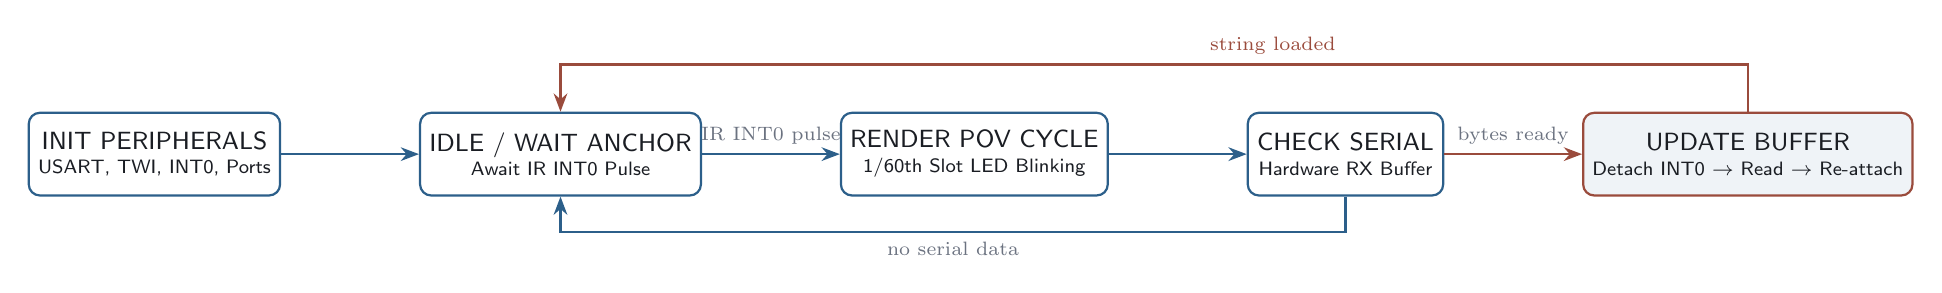
\begin{tikzpicture}[
            node distance=1.75cm,
            state/.style={
                rectangle,
                draw=Accent,
                fill=white,
                thick,
                rounded corners,
                minimum height=1.05cm,
                minimum width=2.45cm,
                align=center,
                font=\sffamily\small,
                text=Ink
            },
            alertstate/.style={
                state,
                draw=Warn,
                fill=AccentSoft
            },
            arrow/.style={-Stealth, thick, color=Accent},
            alertarrow/.style={-Stealth, thick, color=Warn},
            note/.style={font=\scriptsize, color=Dim}
        ]
            \node[state] (init) {INIT PERIPHERALS\\[-2pt]\scriptsize USART, TWI, INT0, Ports};
            \node[state, right=of init] (wait) {IDLE / WAIT ANCHOR\\[-2pt]\scriptsize Await IR INT0 Pulse};
            \node[state, right=of wait] (render) {RENDER POV CYCLE\\[-2pt]\scriptsize 1/60th Slot LED Blinking};
            \node[state, right=of render] (check) {CHECK SERIAL\\[-2pt]\scriptsize Hardware RX Buffer};
            \node[alertstate, right=of check] (detach) {UPDATE BUFFER\\[-2pt]\scriptsize Detach INT0 $\rightarrow$ Read $\rightarrow$ Re-attach};

            % Forward flow
            \draw[arrow] (init) -- (wait);
            \draw[arrow] (wait) -- node[above, note]{IR INT0 pulse} (render);
            \draw[arrow] (render) -- (check);
            \draw[alertarrow] (check) -- node[above, note]{bytes ready} (detach);

            % Feedback loops
            \draw[arrow] (check.south) -- ++(0,-0.45) -| node[pos=0.25, below, note]{no serial data} (wait.south);
            \draw[alertarrow] (detach.north) -- ++(0,0.60) -| node[pos=0.20, above, note, text=Warn]{string loaded} (wait.north);
        \end{tikzpicture}
    }

    \vspace{0.08cm}
    \begin{itemize}
        \footnotesize
        \item \textbf{Interrupt-Driven Rotation Lock:} The IR sensor output triggers an external interrupt on INT0 at the anchor position, marking the exact $0^\circ$ baseline of each rotation cycle.
        \item \textbf{Angular Division (1/60th Slots):} The ATmega32 divides the measured rotation period into 60 equal angular increments to render 60-position analog clock hands (hour, minute, second) and aligned text characters.
        \item \textbf{Bit-Matrix Column Driver:} Writes column bit-patterns directly to GPIO ports with calibrated delay routines to achieve optimal letter width and spacing without blurring.
        \item \textbf{Serial Collision Decoupling:} When Bluetooth data arrives, INT0 is temporarily detached during the UART string buffer transfer and re-attached immediately after, preventing serial interrupt collisions from corrupting the display cycle.
    \end{itemize}
\end{frame}

% --- SLIDE 11: ROLE OF THE ATMEGA32 - PERIPHERAL UTILIZATION ---
\begin{frame}{4. Role of the ATmega32}{Peripheral Utilization Breakdown}
    \footnotesize
    \begin{itemize}
        \item \textbf{GPIO Port Register Control (PA, PB, PC, PD):} Direct 8-bit parallel writes to drive 24 LEDs simultaneously. Executing single-cycle \texttt{PORT} assignments guarantees microsecond-level LED column switching essential for high-RPM display sharpness.
        \item \textbf{External Interrupt 0 (INT0 / PD2):} Falling-edge trigger from the IR obstacle sensor. Captures rotation phase start instantly, resetting the column index counter and eliminating image rotation drift.
        \item \textbf{Hardware TWI / I$^2$C (PC0 / PC1):} Operates at 100 kHz to communicate with the DS3231 RTC module. Fetches seconds, minutes, and hours data during idle phase gaps.
        \item \textbf{Hardware USART (PD0 / PD1):} Configured for 38400 / 9600 baud wireless serial data reception from HC-05. Uses double-buffered RX interrupts to buffer incoming ASCII strings.
        \item \textbf{Timer0 / Timer1 (16-bit / 8-bit):} Provides precision microsecond timebase for calculating rotation period ($T_{rot}$), column delay times ($\Delta t_{col} = T_{rot} / N_{cols}$), and letter spacing intervals.
    \end{itemize}
\end{frame}

% --- SLIDE 12: IMPLEMENTATION PLAN - MILESTONES ---
\begin{frame}{5. Implementation Plan}{Development Stages \& Milestones}
    \begin{columns}[T]
        \begin{column}{0.48\textwidth}
            \begin{block}{Project Update 1 (Wks 1--3)}
                \footnotesize
                \begin{itemize}
                    \item 1.1 Bare-metal ATmega32 clock, GPIO ports, and timer setup.
                    \item 1.2 IR obstacle sensor integration on INT0 for period measurement.
                    \item 1.3 LED column bit-pattern rendering for single static characters ('S', 'A', digits).
                    \item 1.4 Mechanical motor balancing and basic rotating panel assembly.
                \end{itemize}
                \textbf{Deliverable:} Rotating panel displays a steady single character locked to the IR anchor position without drift.
            \end{block}
        \end{column}
        \begin{column}{0.48\textwidth}
            \begin{block}{Final Demonstration (Wks 4--6)}
                \footnotesize
                \begin{itemize}
                    \item 2.1 Hardware TWI driver for DS3231 RTC module time sync.
                    \item 2.2 Hardware USART integration for HC-05 Bluetooth dynamic text input.
                    \item 2.3 Implementation of INT0 detach/re-attach serial decoupling routine.
                    \item 2.4 Rendering routines for Analog Clock (60 slots), Digital Clock, and Scrolling Text.
                    \item 2.5 Onboard Li-Ion power circuit integration and final PCB enclosures.
                \end{itemize}
                \textbf{Deliverable:} Complete wireless floating POV display showing live analog/digital clock and Bluetooth text messages.
            \end{block}
        \end{column}
    \end{columns}
\end{frame}

% --- SLIDE 13: IMPLEMENTATION PLAN - TEAM RESPONSIBILITIES ---
\begin{frame}{5. Implementation Plan}{Group Member Responsibilities}
    \begin{columns}[T]
        \begin{column}{0.32\textwidth}
            \begin{block}{Member 1: 2205139}
                \small
                \begin{itemize}
                    \item Firmware Architecture \& Core Timing Logic
                    \item INT0 interrupt anchor handler \& 1/60th angular slot calculation
                    \item INT0 detach/re-attach serial decoupling logic
                \end{itemize}
            \end{block}
        \end{column}
        \begin{column}{0.32\textwidth}
            \begin{block}{Member 2: 2205143}
                \small
                \begin{itemize}
                    \item Hardware, Motor Drive \& Power Systems
                    \item 24-LED rotating PCB fabrication \& motor mounting
                    \item 3.7V Li-Ion battery power regulation \& mechanical balancing
                \end{itemize}
            \end{block}
        \end{column}
        \begin{column}{0.32\textwidth}
            \begin{block}{Member 3: 2205147}
                \small
                \begin{itemize}
                    \item Peripheral Interfaces \& Software Utility
                    \item DS3231 RTC TWI driver \& HC-05 USART driver
                    \item Character bit-matrix encoding \& mobile Bluetooth terminal testing
                \end{itemize}
            \end{block}
        \end{column}
    \end{columns}
\end{frame}

% --- SLIDE 14: USE OF OTHER CONTROLLERS ---
\begin{frame}{6. Use of Other Controllers}{Controller Selection \& Arduino Nano Replacement Justification}
    \begin{block}{Main System Architecture}
        \scriptsize The \textbf{ATmega32-16PU} serves as the sole central controller for the entire project. It directly manages the IR phase anchor interrupt, DS3231 RTC TWI bus, HC-05 Bluetooth USART communication, and 24-LED array port drivers.
    \end{block}
    \vspace{-0.1cm}
    \begin{block}{Evaluation of Secondary / External Controllers}
        \scriptsize
        \begin{itemize}
            \item \textbf{Why Arduino Nano was initially considered:} Popular dev-board choice in early prototyping due to integrated USB-to-serial chip and ready-made header pins.
            \item \textbf{Is Arduino Nano strictly mandatory?} \textbf{NO.} It is an ATmega328P breakout board. Replacing it with the ATmega32 results in \textbf{zero feature loss} and improves hardware design.
            \item \textbf{Why ATmega32 is Superior for this Project:}
                \begin{itemize}
                    \tiny
                    \item \textbf{Direct 8-Bit Port Manipulation:} ATmega32 has 32 I/O lines across 4 clean 8-bit ports (PA, PB, PC, PD). All 24 LEDs connect directly to full ports, enabling instant 1-cycle \texttt{PORT} writes for sharp LED column switching.
                    \item \textbf{Fixes Clone Nano Baud Rate Bug:} Eliminates the hardware baud rate mismatch observed on cloned Nano boards (where 38400 baud operated at 9600 due to bad fuses/crystals). Using ATmega32 with an 11.0592 MHz crystal gives 0.0\% baud error.
                    \item \textbf{No Auxiliary Controllers Required:} No ESP32 or Raspberry Pi is needed. ATmega32 alone possesses sufficient memory, timers, and hardware peripherals to execute all tasks autonomously.
                \end{itemize}
        \end{itemize}
    \end{block}
\end{frame}

% --- SLIDE 15: TESTING AND SUCCESS CRITERIA ---
\begin{frame}{7. Testing \& Success Criteria}{Measurable Criteria \& Test Methodology}
    \tiny
    \renewcommand{\arraystretch}{0.88}
    \begin{table}
        \centering
        \begin{tabular}{p{2.5cm} p{2.5cm} p{5.5cm} p{1.1cm}}
            \toprule
            \textbf{\color{Accent} Metric} & \textbf{\color{Accent} Target Value} & \textbf{\color{Accent} Test Method \& Validation Tool} & \textbf{\color{Accent} Priority} \\
            \midrule
            Phase Sync Stability & 0$^\circ$ image rotation drift & Visual inspection under stroboscopic/steady rotation over 10 minutes & Essential \\
            Frame Refresh Rate & $\ge 20$ Hz ($\ge 1200$ RPM) & DC motor tachometer check; ensures flicker-free human vision retention & Essential \\
            Interrupt Latency & $< 5\,\mu$s on INT0 & Oscilloscope check from IR sensor pulse edge to ISR execution start & Essential \\
            LED Column Switch Speed & $< 1\,\mu$s per column & Direct \texttt{PORT} write execution check on logic analyzer & Essential \\
            Bluetooth Transmission & 100\% ASCII string integrity & Send 50-character strings via Serial Bluetooth Terminal at 38400 baud & Essential \\
            RTC Time Synchronization & $\pm 1$ second precision & Compare displayed analog/digital clock hands against DS3231 hardware RTC & Essential \\
            Serial Decoupling Safety & Zero display glitching during RX & Send continuous Bluetooth text streams while POV rendering is active & Essential \\
            Power Battery Autonomy & $\ge 45$ minutes continuous & 3.7V Li-Ion discharge test under full 24-LED spinning load & Essential \\
            Wireless Control GUI & Smartphone app interface & Optional custom Android app with buttons for mode switching & Optional \\
            \bottomrule
        \end{tabular}
    \end{table}
    \vspace{0.15cm}
    \footnotesize\color{Dim} Essential features: INT0 phase locking, 24-LED PORT driving, DS3231 RTC clock sync, HC-05 USART text reception, and serial decoupling. Optional features: Custom smartphone UI app.
\end{frame}

% --- SLIDE 16: CHALLENGES AND FUTURE SCOPE ---
\begin{frame}{8. Challenges \& Future Scope}{Anticipated Technical Issues \& Scaling Path}
    \begin{columns}[T]
        \begin{column}{0.48\textwidth}
            \begin{block}{Technical Challenges \& Solutions}
                \tiny
                \begin{itemize}
                    \item \textbf{Bluetooth Baud Rate Mismatch:} Cloned Arduino Nanos showed baud rate errors (38400 settings acting as 9600) $\rightarrow$ \textbf{Solution:} Switch to ATmega32 with dedicated 11.0592 MHz crystal for exact 0.0\% UART baud calculation.
                    \item \textbf{Sensor Jitter (Hall vs IR):} Hall magnetic sensor signals proved jittery and imprecise $\rightarrow$ \textbf{Solution:} Replaced with an IR obstacle sensor, providing clean digital pulses for INT0 anchor locking.
                    \item \textbf{Timing vs Interrupt Drift:} Periodic timing alone caused continuous image rotation $\rightarrow$ \textbf{Solution:} Re-synchronized display loop on every rotation cycle using INT0 falling-edge interrupt.
                    \item \textbf{Serial-Display Collision:} Receiving Bluetooth data inside ISR caused display overlap $\rightarrow$ \textbf{Solution:} Temporarily detach INT0 interrupt during UART string reading, then re-attach immediately after buffer update.
                    \item \textbf{Letter Spacing \& Column Timing:} Blur occurs if LED ON-time is improperly calibrated $\rightarrow$ \textbf{Solution:} Microsecond-level timer delay calibration based on real-time $T_{rot}$.
                \end{itemize}
            \end{block}
        \end{column}
        \begin{column}{0.48\textwidth}
            \begin{block}{Future Scope}
                \tiny
                \textbf{Near-Term Enhancements}
                \begin{itemize}
                    \item \textbf{Wireless Power Transfer / Slip Rings:} Implement inductive wireless power coils on the motor base to eliminate Li-Ion battery recharging downtime.
                    \item \textbf{RGB Full-Color LEDs:} Upgrade 24 mono LEDs to WS2812B / APA102 RGB LEDs to render full-color graphics and animations.
                \end{itemize}
                \textbf{Long-Term Scaling}
                \begin{itemize}
                    \item \textbf{3D Holographic Display:} Stagger multiple rotating vertical LED arcs at offset angles to create full 3D volumetric holographic projections.
                    \item \textbf{Dedicated Mobile App GUI:} Build a custom Android/iOS app with visual drawing canvas to stream real-time doodles directly to the display over Bluetooth.
                \end{itemize}
            \end{block}
        \end{column}
    \end{columns}
\end{frame}

\end{document}
